\documentclass[a4paper, 14pt]{extreport}
\usepackage[T2A]{fontenc}
\usepackage[utf8x]{inputenc}
\usepackage[english, russian]{babel}
\usepackage{indentfirst}
\usepackage{amssymb, amsthm, amsfonts, amsmath, mathtext, wasysym}
\usepackage{cite, enumerate, float}
\usepackage{graphicx}
\usepackage{multicol, multirow, array}
\usepackage{times}
\usepackage{geometry}
\usepackage{setspace}
\usepackage{titlesec}
\usepackage[square, numbers, sort&compress]{natbib}
\usepackage{tocloft}
\usepackage{caption}
\usepackage{listings}
\usepackage{fancyhdr}
\usepackage[colorlinks, linkcolor=black, citecolor=black, urlcolor=blue]{hyperref}
\usepackage{algorithm2e}
\geometry{left=2.0cm}
\geometry{right=1.5cm}
\geometry{top=2.0cm}
\geometry{bottom=2.0cm}
\graphicspath{{images/},{plots/}}

% use Times New Roman for text
\renewcommand{\rmdefault}{ftm}
\lstset{
    language=C++,
    extendedchars=\true,
    inputencoding=utf8,
    basicstyle=\scriptsize\usefont{T2A}{fcr}{m}{n},
    keywordstyle=\bfseries,
    commentstyle=\itshape,
    numbers=left,
    numberstyle=\tiny,
    breakatwhitespace=\false,
    breaklines=\true,
    tabsize=2, 
}

% fancyhdr page style
\pagestyle{fancy}
\fancyhf{}
\fancyhead[R]{\thepage}
\fancyheadoffset{0mm}
\fancyfootoffset{0mm}
\setlength{\headheight}{17pt}
\renewcommand{\headrulewidth}{0pt}
\renewcommand{\footrulewidth}{0pt}
\fancypagestyle{plain}{
    \fancyhf{}
    \rhead{\thepage}
}

% title style
\titleformat{\chapter}
    {\centering\normalsize}
    {\thechapter}
    {8pt}{\MakeUppercase}
\titleformat{\section}
    {\centering\normalsize}
    {\thesection}
    {1em}{}
\titleformat{\subsection}
    {\centering\normalsize}
    {\thesubsection}
    {1em}{}
  
\titlespacing*{\chapter}{0pt}{-30pt}{8pt}
\titlespacing*{\paragraph}{0pt}{-30pt}{8pt}
\titlespacing*{\section}{\parindent}{*4}{*4}
\titlespacing*{\subsection}{\parindent}{*4}{*4}

\makeatletter

\renewcommand{\@biblabel}[1]{#1} 

% bibliography bibitem item indent
\renewenvironment{thebibliography}[1]
    {\chapter*{\bibname}%
    \@mkboth{\MakeUppercase\bibname}{\MakeUppercase\bibname}%
    \list{\@biblabel{\@arabic\c@enumiv}}%
        {\settowidth\labelwidth{\@biblabel{#1}}%
        \leftmargin=0pt
        \itemindent=50pt
        \@openbib@code
        \usecounter{enumiv}%
        \let\p@enumiv\@empty
        \renewcommand\theenumiv{\@arabic\c@enumiv}}%
    \sloppy
    \clubpenalty4000
    \@clubpenalty \clubpenalty
    \widowpenalty4000%
    \sfcode`\.\@m}
        {\def\@noitemerr
        {\@latex@warning{Empty `thebibliography' environment}}%
    \endlist}
    
\makeatother

\newcolumntype{C}[1]{>{\centering\arraybackslash}m{#1\textwidth}}
\renewcommand{\arraystretch}{1.2}

\DeclareCaptionLabelFormat{figure}{Рисунок #2}
\DeclareCaptionLabelFormat{table}{Таблица #2}
\DeclareCaptionLabelSeparator{sep}{~---~}
\captionsetup{labelsep=sep, justification=centering, font=small}
\captionsetup[figure]{labelformat=figure}
\captionsetup[table]{labelformat=table}

\renewcommand{\cfttoctitlefont}{\normalfont\hspace{0.38\textwidth}}
\renewcommand{\cftbeforetoctitleskip}{-1em}
\renewcommand{\cftchapfont}{\normalsize}
\renewcommand{\cftsecfont}{\hspace{-21pt}}
\renewcommand{\cftsubsecfont}{\hspace{-53pt}}
\renewcommand{\cftbeforechapskip}{0em}
\renewcommand{\cftparskip}{-1mm}
\renewcommand{\cftdotsep}{1}
\renewcommand{\cftsecpresnum}{}
\renewcommand{\cftchapleader}{\cftdotfill{\cftdotsep}}
\renewcommand{\cftsecleader}{\cftdotfill{\cftdotsep}}
\renewcommand{\cftsecaftersnum}{.}
\renewcommand{\cftsubsecaftersnum}{.}
\setcounter{tocdepth}{2}

\renewcommand{\theenumi}{\arabic{enumi}}
\renewcommand{\labelenumi}{\arabic{enumi})}
\renewcommand{\theenumii}{.\arabic{enumii}}
\renewcommand{\labelenumii}{\arabic{enumi}.\arabic{enumii})}
\renewcommand{\theenumiii}{.\arabic{enumiii}}
\renewcommand{\labelenumiii}{\arabic{enumi}.\arabic{enumii}.\arabic{enumiii})}

\newcommand{\pder}[2] {\frac{\partial #1}{\partial #2}}
% частная производная от #1 по #2
\newcommand{\ppder}[2]{\frac{\partial^2 #1}{\partial {#2}^2}}
% вторая частная производная от #1 по #2
\newcommand{\pcder}[3]{\frac{\partial^2 #1}{\partial #2 \partial #3}}
% вторая частная производная от #1 по #2 и #3
\newcommand{\der}[2]  {\frac{d #1}{d #2}}
% производная от #1 по #2
\newcommand{\dder}[2] {\frac{d^2 #1}{d {#2}^2}}
% вторая производная от #1 по #2
\newcommand{\abs}[1]{\left| #1 \right|}
% обозначение модуля

% Перевод плагина algorithm2e
\SetKwInput{KwData}{Исходные параметры}
\SetKwInput{KwResult}{Результат}
\SetKwIF{If}{ElseIf}{Else}{если}{тогда}{иначе\ если}{иначе}{конец\ условия}
\SetKwFor{While}{до\ тех\ пор,\ пока}{выполнять}{конец\ цикла}
\SetAlgorithmName{Алгоритм}{алгоритм}{Список алгоритмов}

\addto{\captionsrussian}{\renewcommand*{\contentsname}{СОДЕРЖАНИЕ}}

\begin{document}
    \onehalfspacing
    \begin{titlepage}
	\begin{center}
		Министерство образования и науки РФ \\
		\vspace{.5cm}
		ГОСУДАРСТВЕННОЕ ОБРАЗОВАТЕЛЬНОЕ УЧРЕЖДЕНИЕ\\*
		ВЫСШЕГО ПРОФЕССИОНАЛЬНОГО ОБРАЗОВАНИЯ\\*
		<<ВОЛГОГРАДСКИЙ ГОСУДАРСТВЕННЫЙ ТЕХНИЧЕСКИЙ УНИВЕРСИТЕТ>>\\
		\vspace{.5cm}
		Кафедра <<ФИЗИКА>>
		\vspace{.5cm}
	\end{center}
	\begin{flushright}
		УТВЕРЖДАЮ\\
		Заведующий кафедрой <<Физика>>\\
		\vspace{.3cm}
		\underline{\hspace{2cm}}\hspace{1cm}\underline{\hspace{4cm}}\\
		\vspace{-.2cm}\footnotesize(подпись)\hspace{1.8cm}(инициалы, фамилия)
			\hspace*{.2cm}\ \normalsize\\
		\vspace{.3cm}
		<<\underline{\ \ \ \ }>>\underline{\ \ \ \ \ \ \ \ \ \ \ \ \ \ } 
			\the\yearг.
	\end{flushright}
	\begin{center}
		\LARGE \textbf{ПОЯСНИТЕЛЬНАЯ ЗАПИСКА} \\
		\large К ВЫПУСКНОЙ РАБОТЕ БАКАЛАВРА
	\end{center}
	\begin{center}
		на тему \underline{моделирование структуры абрикосовских вихрей в 
        	сверхпроводниках типа 1,5}
	\end{center}
	\begin{flushleft}
		Автор\hspace{2.5cm}Голубев~А.~В.\hfill\underline{\hspace{5cm}}\\
		\vspace{-.2cm}\hspace{14cm}\footnotesize(подпись, дата)\normalsize\\
		\vspace{-.5cm}
		Группа\hspace{2.2cm}Ф-469\\
		Направление\hspace{1cm}010700.62\\
		Руководитель работы (проекта)\\
		\underline{д. ф.-м. н., Завьялов~Д.~В.}\hfill\underline{\hspace{5cm}}\\
		\vspace{-.2cm}\hspace{.4cm}\footnotesize(уч. звание, уч. степень, 
			фамилия, инициалы)\hspace{6.5cm}(подпись, дата)\normalsize\\
		Консультанты\\
		по научной части \underline{\hspace{7cm}}\hfill%
			\underline{\hspace{5cm}}\\\vspace{-.2cm}\hspace{4cm}%
			\footnotesize(уч. звание, уч. степень, фамилия, инициалы)%
			\hspace{3cm}(подпись, дата)\normalsize\\
		Нормоконтроллер \underline{\hspace{7cm}}
			\hfill\underline{\hspace{5cm}}\\
		\vspace{-.2cm}\hspace{4cm}\footnotesize(уч. звание, уч. степень, 
			фамилия, инициалы)\hspace{3cm}(подпись, дата)\normalsize\\
	\end{flushleft}

	\vspace{\fill}

	\begin{center}
		Волгоград \the\year
	\end{center}
\end{titlepage}

\begin{titlepage}
	\begin{center}
		Министерство образования и науки РФ \\
		\vspace{.5cm}
		ГОСУДАРСТВЕННОЕ ОБРАЗОВАТЕЛЬНОЕ УЧРЕЖДЕНИЕ\\*
		ВЫСШЕГО ПРОФЕССИОНАЛЬНОГО ОБРАЗОВАНИЯ\\*
		<<ВОЛГОГРАДСКИЙ ГОСУДАРСТВЕННЫЙ ТЕХНИЧЕСКИЙ УНИВЕРСИТЕТ>>\\
		\vspace{.5cm}
		Кафедра <<ФИЗИКА>>
		\vspace{.5cm}
	\end{center}
	\begin{flushright}
		УТВЕРЖДАЮ\\
		Заведующий кафедрой <<Физика>>\\
		\vspace{.3cm}
		\underline{\hspace{2cm}}\hspace{1cm}\underline{\hspace{4cm}}\\
		\vspace{-.2cm}\footnotesize(подпись)\hspace{1.8cm}(инициалы, фамилия)
			\hspace*{.2cm}\ \normalsize\\
		\vspace{.3cm}
		<<\underline{\ \ \ \ }>>\underline{\ \ \ \ \ \ \ \ \ \ \ \ \ \ } 
			\the\yearг.
	\end{flushright}
	\begin{center}
		\large Задание \\
		\normalsize на выпускную работу бакалавра
	\end{center}
	\begin{flushleft}
		Студент Голубев Алексей Владимирович\\
		Код кафедры \underline{\hspace{3cm}}\hspace{6cm}Группа Ф-469\\
		Тема <<Моделирование структуры абрикосовских вихрей в сверхпроводниках 
		    типа 1,5>>\\
		Утверждена приказом по ВолгГТУ от <<\underline{\hspace{1cm}}>> октября 2013г. №\underline{\hspace{3.5cm}}\\
		Срок представления готовой работы \underline{\hspace{6cm}}\\
		\vspace{-.2cm}\hspace{9.5cm}\footnotesize(дата, подпись студента)
			\normalsize\\
		\vspace{.3cm}
		Исходные данные для выполнения работы (проекта)\\
		\hrulefill\\
		\hrulefill\\
		\hrulefill\\
		\hrulefill\\
		Содержание основной части пояснительной записки\\
		\hrulefill\\
		\hrulefill\\
		\hrulefill\\
		\hrulefill\\

		\begin{center}
	    	Перечень графического материала\\
		\end{center}
		1) \hrulefill\\
		\hrulefill\\
		2) \hrulefill\\
		\hrulefill\\
		3) \hrulefill\\
		\hrulefill\\
		4) \hrulefill\\
		\hrulefill\\
		5) \hrulefill\\
		\hrulefill\\
		6) \hrulefill\\
		\hrulefill\\
		7) \hrulefill\\
		\hrulefill\\
		8) \hrulefill\\
		\hrulefill\\
		9) \hrulefill\\
		\hrulefill\\
		10) \hrulefill\\
		\hrulefill\\
		11) \hrulefill\\
		\hrulefill\\

		Руководитель работы (проекта) \underline{\hspace{5cm}}%
			\hfill\underline{\hspace{4cm}}\\
		\vspace{-.2cm}\hspace{7.3cm}\footnotesize(подпись и дата подписания)%
			\hspace{2.2cm}(инициалы и фамилия)\normalsize\\
		Консультанты по разделам:\\
		\underline{\hspace{7.5cm}}\hspace{1cm}\underline{\hspace{4cm}}%
			\hspace{1cm}\underline{\hspace{4cm}}\\
		\vspace{-.2cm}\hspace{1.5cm}\footnotesize(краткое наименование раздела)%
			\hspace{2cm}(подпись и дата подписания)%
			\hspace{1.1cm}(инициалы и фамилия)\normalsize\\
		\underline{\hspace{7.5cm}}\hspace{1cm}\underline{\hspace{4cm}}%
			\hspace{1cm}\underline{\hspace{4cm}}\\
		\vspace{-.2cm}\hspace{1.5cm}\footnotesize(краткое наименование раздела)%
			\hspace{2cm}(подпись и дата подписания)%
			\hspace{1.1cm}(инициалы и фамилия)\normalsize\\
		\underline{\hspace{7.5cm}}\hspace{1cm}\underline{\hspace{4cm}}%
			\hspace{1cm}\underline{\hspace{4cm}}\\
		\vspace{-.2cm}\hspace{1.5cm}\footnotesize(краткое наименование раздела)%
			\hspace{2cm}(подпись и дата подписания)%
			\hspace{1.1cm}(инициалы и фамилия)\normalsize\\
		\underline{\hspace{7.5cm}}\hspace{1cm}\underline{\hspace{4cm}}%
			\hspace{1cm}\underline{\hspace{4cm}}\\
		\vspace{-.2cm}\hspace{1.5cm}\footnotesize(краткое наименование раздела)%
			\hspace{2cm}(подпись и дата подписания)%
			\hspace{1.1cm}(инициалы и фамилия)\normalsize\\
	\end{flushleft}
	\thispagestyle{empty}
\end{titlepage}
\setcounter{page}{4}
    % переработать тексты
\tocless\part{Аннотация}
Развитие городов сопряжено с модернизацией существующей сети общественного транспорта. Современные 
коммуникационные технологии позволяют собирать данные о перемещениях людей в городской среде, на основе 
которых можно сделать выводы о предпочтениях людей по перемещению внутри городской среды. Фактически, 
подобные предпочтения можно рассматривать как требования к структуре сети общественного транспорта. 
Имея данные о ежедневных передвижениях людей, мы можем понять реальные предпочтения и потребности людей 
в системе городского транспорта. Следовательно, может быть предложена модификация транспортной сети или 
даже набор возможных альтернатив. Эта модификация отражает реальные потребности людей и сокращает время 
передвижения и повышает общий уровень удовлетворенности. Однако для решением задача анализа 
геопространственных данных необходимо получить набор субоптимальных маршрутов для выбора. Получение 
оптимальных маршрутов сети является повторяющейся процедурой, которая требует вмешательство эксперта.
В данной работе предлагаются методы, позволяющий на основе данных о предпочтениях пользователей 
общественного транспорта формировать схему маршрутов общественного транспорта.

Список ключевых слов: геоданные, транспортная сеть, транспорт, генетические алгоритмы, 
алгоритмы оптимизации, итерационные алгоритмы, \ldots

\tocless\part{Abstract}
Urban development is connected with the existing public transportation network modernization. Modern 
communication technologies make it possible to collect data on the movements of people in the urban 
environment, based on which is possible to draw conclusions about people's preferences on the movement 
inside the urban space. In fact, these preferences may be considered as requirements for the public 
transportation network. Having data about people's everyday movements, we can understand the real 
people preferences and needs in the urban transport system. Hence, as the results of analysis the 
modified transport network (or even a bunch of alternative) can be suggested. This new solutions reflects 
real people needs and reduce transfer time and increase satisfaction level. However the problem of 
geospatial data analysis is need to be solved to get (sub)optimal routes for choosing by authorities. 
Getting optimal routes network is an iterative procedure which requires human (expert) intervention.
The proposed methods allows to create a public transportation routes scheme based on data about the 
public transportation users preferences.

List of keywords: geodata, transport network, transport, genetic algorithms, optimization algorithms,
iterative algorithms, \ldots
    \tableofcontents
    \newpage
    \begin{center}
	ОПРЕДЕЛЕНИЯ, ОБОЗНАЧЕНИЯ И СОКРАЩЕНИЯ
\end{center}

В настоящей работе применяют следующие термины с соответствующими определениями:
\begin{itemize}
    \item ТГЛ -- теория Гинзбурга-Ландау
    \item ГЛ -- Гинзбург-Ландау
    \item БКШ -- Бардин - Купер - Шриффер
\end{itemize}

\newpage
    \chapter*{Введение}
\addcontentsline{toc}{chapter}{Введение}

В последнее время наблюдается повышенный интерес к сверхпроводникам с 
несколькими сверхпроводящими компонентами. Основные ситуации, когда возникают 
множественные сверхпроводящие компоненты: многозонные сверхпроводники второго 
рода \cite{bib:6,bib:7,bib:8,bib:9,bib:10,bib:11}, сверхпроводимость первого 
рода в смеси независимых консервативных конденсатов, таких как прогнозируемая 
сверхпроводимость в атомарном водороде и богатых водородом сплавов 
\cite{bib:12.1,bib:12.2,bib:13,bib:14} и сверхпроводников с другим типом 
симметрии, отличной от поперечно-волновой симметрии. Интерес к исследованию 
вихревого состояния обусловлен широкими потенциальными возможностями 
применения сверхпроводников в современной микроэлектронике и энергетике, а 
также интересом к самой физике процессов происходящих в смешанном состоянии 
сверхпроводников. Развитие нанотехнологии и открытие новых сверхпроводящих 
соединений (в частности, высокотемпературных сверхпроводников) стимулировали 
новые теоретические и экспериментальные исследования смешанного состояния. 

В работе проведено исследование появления сверхпроводимости 1,5-го рода с 
акцентом на случай многополосной сверхпроводимости, демонстрируя сохранение 
этого типа сверхпроводимости в присутствии различных видов межкомпонентных 
соединений (например, межзонное джозефсоновской связи, смешанных градиентных 
связей, связи типа плотность-плотность, и других видов).

\textbf{Актуальность.}

Главным фактором в изучении явления сверхпроводимости является временные 
затраты на проведение модельных экспериментов. Поэтому для решения 
поставленных задач нужно использовать более быстрые и эффективные алгоритмы.

\textbf{Методы исследования.}

Достоверность результатов обеспечена оптимальным выбором физических моделей, 
учитывающих основные свойства исследуемых систем, и адекватным выбором метода 
численного моделирования.

\textbf{Научная новизна.}

С целью использования градиентных алгоритмов минимизации (типа LBFGS), для 
которых знание градиента минимизируемой функции в явном виде является 
желательным условием, был использован метод автоматического дифференцирования 
(библиотека CppAD). Для минимизации функционала свободной энергии в модели 
Гинзбурга -- Ландау впервые был использован алгоритм LBFGS.

\textbf{Научная и практическая значимость.}

Используемый алгоритм Бройдена -- Флетчера -- Гольдфарба -- Шанно сокращает
временные затраты на минимизацию функционала Гинзбурга -- Ландау по сравнению 
с другими методами.

\newpage
    \section{Основные характеристики сверхпроводящего состояния}

Теория и эксперимент показывают, что лондоновская глубина проникновения 
\( \lambda \), длина когерентности \( \xi \) и энергетическая щель 
\( \Delta \) не являются константами, а зависят от температуры и обладают 
сугубо индивидуальными для заданного материала величинами. Величины 
\( \lambda \) и \( \xi \) имеют минимальное значение при \( T = 0 \) и 
монотонно возрастают с увеличением температуры, стремясь к бесконечности при 
\( T = T_c \) (это объясняется тем, что выше критической температуры никаких 
куперовских пар нет, а магнитное поле беспрепятственно пронизывает вещество). 
Энергетическая щель \( \Delta \), наоборот, имеет максимум при \( T = 0 \) и 
становится равной нулю при \( T = T_c \) (что можно трактовать как отсутствие 
каких-либо корреляций между электронами).

Теория БКШ дает исчерпывающее описание сверхпроводящих свойств материала во 
всём температурном интервале от \( 0 \) до \( T_c \), но является сложной с 
математической точки зрения. Поэтому часто физики прибегают к другому, 
относительно более простому способу анализа сверхпроводящего состояния -- ТГЛ, 
которая прекрасно описывает, качественно и количественно, поведение 
сверхпроводника, но работает только в ограниченном интервале вблизи 
критической температуры.

Теория Гинзбурга–Ландау основывается на теории фазовых переходов 2-го рода. В 
этой теории, наряду с критической температурой, длиной когерентности и 
лондоновской глубиной проникновения, вводится еще одна характеристика, -- 
параметр порядка. С точностью до некоторого коэффициента пропорциональности 
можно считать, что модуль параметра порядка -- это энергетическая щель в 
теории БКШ. Параметр порядка равен нулю при \( T = T_c \) и выше и принимает 
максимальное значение, когда температура достигла абсолютного нуля. Отметим, 
что есть и иная трактовка физического смысла параметра порядка: квадрат его 
модуля определяет концентрацию куперовских пар.

Параметр порядка играет ключевую роль в теории Гинзбурга–Ландау. Через него 
выражается энергия (с точки зрения термодинамики корректнее говорить 
свободная энергия) сверхпроводника.\cite{bib:net}

\section{Сверхпроводимость 1-го и 2-го рода}

Несмотря на то что теория Гинзбурга–Ландау является феноменологической, то 
есть она не объясняет причины возникновения явления, которое она описывает, с 
ее помощью был получен ряд важных результатов. Применив эту теорию, ее авторы 
вычислили поверхностную энергию, возникающую на границе сверхпроводника и 
нормального металла в присутствии внешнего магнитного поля. Оказалось, что 
результат зависит от безразмерной величины, называемой параметром 
Гинзбурга–Ландау \( \kappa \): \( \kappa = \lambda/\xi \) (отношение 
лондоновской глубины проникновения к длине когерентности). Из расчетов 
следовало, что при \( \kappa < 1/\sqrt{2} \) поверхностная энергия оказывается 
положительной. Для сверхпроводника цилиндрической формы, ось которого 
параллельна силовым линиям магнитного поля, данный результат означал, что 
переход в нормальное состояние происходит моментально, как только индукция 
магнитного поля превышает некоторое критическое значение \( B_c \) для данной 
температуры (рис. 1). В принципе, ничего нового Гинзбург и Ландау не получили, 
они лишь теоретически подтвердили хорошо известный уже на тот момент 
экспериментальный факт поведения сверхпроводников.

Советский физик Николай Заварицкий, исследуя тонкие сверхпроводящие пленки, 
обнаружил, что их поведение в магнитном поле не согласуется с предсказаниями 
теории Гинзбурга–Ландау. Чтобы понять причину расхождения, Алексей Абрикосов, 
основываясь на теории Гинзбурга–Ландау, решил рассмотреть случай, когда 
поверхностная энергия является отрицательной, -- иными словами, попытаться 
понять картину поведения сверхпроводника в магнитном поле с 
\( \kappa > 1/\sqrt{2} \).

Из расчетов следовало, что пока индукция магнитного поля не превосходит нижнее 
критическое значения поля \( B_{c1} \) при фиксированной температуре, 
сверхпроводник находится в мейсснеровском состоянии. После того как индукция 
магнитного поля стала больше \( B_{c1} \), сверхпроводник начинают пронизывать 
своеобразные нити микронных размеров, вытянутые вдоль силовых линий внешнего 
поля. Чем больше индукция поля, тем больше ниток будет в сверхпроводнике. 
Абрикосов установил, что эти образования представляют собой вихри (теперь они 
называются абрикосовскими), ядра которых являются несверхпроводящими, 
нормальными, с размером порядка длины когерентности \( \xi \), а вокруг них 
протекают циркулирующие сверхпроводящие токи, которые экранируют нормальную 
область вихря (ширина области экранировки равна лондоновской глубине 
проникновения \( \lambda \)). Кроме того, в ходе вычислений обнаружилось, что 
вихри несут в себе как бы одну силовую линию внешнего магнитного поля, или 
квант магнитного потока, флюксоид 
\( \Phi_0 = h/2e = 2,07\cdot10^{–15} \text{Тл}\cdot{м}^2 \). Вихри формируют в 
сверхпроводнике треугольную решетку, образуя смешанное (оно же вихревое) 
состояние (рис. 1).

Если при заданной температуре продолжить усиливать магнитное поле, то при 
верхнем критическом значении \( B_{c2} \) вихрей станет настолько много, что 
их ядра начнут перекрываться, и они заполнят весь объем сверхпроводника, 
переводя его в нормальное состояние (рис. 1).\cite{bib:net}

\section{Сверхпроводимость 1,5-го рода и двухщелевые сверхпроводники}
В 2001 году в дибориде магния \( MgB_2 \) была открыта сверхпроводимость с 
неожиданно высокой критической температурой 39 К. Применяя различные 
экспериментальные техники, ученые установили, что большое значение \( T_c \) 
достигается за счет наличия в \( MgB_2 \) не одной энергетической щели, а 
двух. То есть в сверхпроводящем дибориде магния присутствует как бы два сорта 
куперовских пар. Их взаимодействие и обеспечивает высокую \( T_c \). Важно 
отметить, что у каждого сорта электронных пар есть свой размер, или своя длина 
когерентности. При этом диборид магния имеет лишь одну величину лондоновской 
глубины проникновения.

Возможность нового типа сверхпроводимости, отличного от первого и второго рода 
в многокомпонентных системах \cite{bib:1,bib:2} основана на следующих 
соображениях. Краевая задача в уравнении типа Гинзбурга-Ландау в присутствии 
оборота фазы сводится к одномерной задачи в целом. Кроме того, как указано в 
\cite{bib:1,bib:2}, в общей двухкомпонентной модели есть три фундаментальные 
масштабные длины, которые указывают на невозможно параметризовать модель с 
точки зрения одного безразмерного параметра \( \kappa \). В случае, когда 
конденсаты не связаны межзонной джозефсоновской связью, при условии, что 
векторный потенциал этих масштабных длин представлен двумя независимыми 
величинами: длиной когерентности (устанавливается обратной массой 
соответствующей плотности скалярного поля) и глубиной проникновения магнитного 
поля (устанавливается обратной массой полученного калибровочного поля). В 
противоположность этому, в случае, когда конденсаты соединяются с межзонными 
Джозефсоновскими условиями, можно не различить независимые длины когерентности 
и отнести их к различным конденсатам. Тем не менее, в этом случае колебания 
плотности также могут обладать двумя основными пространственными длинами
\cite{bib:2}, в отличие от однокомпонентных теорий. В \cite{bib:1,bib:2} 
вихревых решениях в двухкомпонентной теории были найдены компоненты, которые 
имеют немонотонное вихревое взаимодействие, с доминирующими частями отвечающие 
за дальнодействующее плотность-плотность взаимодействие и отталкивающей части 
близкодействия типа ток-ток, и электромагнитного взаимодействия. Важным 
обстоятельством, которое было продемонстрировано, что эти вихри 
термодинамически стабильны, несмотря на существование притягивающего хвоста во 
взаимодействии.

\begin{figure}[h!]
  \center
  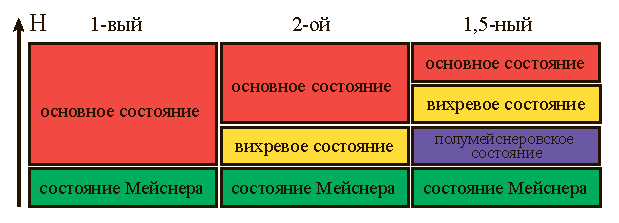
\includegraphics[width=.8\textwidth]{1-01}
  \caption{Сравнение фазовых диаграмм магнитных фаз чистых сверхпроводников
    первого, второго и полуторного рода при нулевой температуре. В 
    полумейсснеровском режиме макроскопическое разделение фаз в 
    двухкомпонентном Мейсснеровском состоянии и вихревых скоплений, где один 
    из режимов плотности подавляется внутренним перекрытием.}
  \label{fig:1}
\end{figure}

Немонотонный межвихревой потенциал взаимодействия должен привести к 
образованию вихревых скоплений в слабомагнитном поле, погруженного в 
безвихревые пространство, эффект упомянутый в \cite{bib:1} как 
"полумейсснеровское состояние". На рисунке \ref{fig:1} схематические показана 
фазовая диаграмма сверхпроводника тип 1,5.

Если вихри образуют кластеры, то нельзя не использовать обычный одномерный 
аргумент относительно энергии сверхпроводника в нормальном состоянии границы 
раздела(!) для классификации магнитного отклика системы. Прежде всего, энергия 
на вихрь в таком случае зависит от того, находится ли вихрь в кластере или 
нет: т.е. формирование единого изолированного вихря может быть энергетически 
невыгодным, в то время как формирование вихревых кластеров выгодно, потому что 
в кластере, где помещены вихри -- минимум потенциала взаимодействия, энергия 
на квант потока меньше, чем для изолированного вихря (термодинамически 
немонотонный потенциал взаимодействия двух вихрей предусматривает, что 
наименьшей энергией на квант потока будет в случае равномерной сетки с шагом 
равным не менее двухчастичного межвихревого потенциала).

Таким образом, помимо энергии вихря в кластере, появляется дополнительная 
энергическая характеристика, связанная с границей кластера. Другими словами, в 
этой ситуации, для определения магнитного отклика системы недостаточно 
изучения краевой задачи и задачи одиночного вихря, в отличии от системы 
отдельных составляющих. В кластере система стремится к минимуму граничной 
энергии (так же, как и в сверхпроводниках 1-го рода), в то время нарушение 
структуры одного квантового вихря внутри кластера (аналогично 
сверхпроводимости второго рода с отрицательной энергией межфазного 
взаимодействия). Таким образом, увеличение магнитного поля образуется 
посредством фазового перехода первого рода. Магнитная фаза отлична от вихря в 
мейснеровском состоянии, затем возникает макроскопическое фазовое 
распределение в двухкомпонентной области Мейснера и вихревых кластерах, где 
один из режимов плотностей подавляется основным перекрытием.\cite{bib:main}

\newpage
    \chapter{Теоретический анализ модели}

\section{Функционал свободной энергии}

Сверхпроводимость 1,5-го рода изучается с помощью следующего двухкомпонентного 
функционала свободной энергии Гинзбурга-Ландау:
\begin{gather}
    F = \frac{1}{2}(D\psi_1)(D\psi_1)^* + \frac{1}{2}(D\psi_2)(D\psi_2)^* - 
        \nu Re\left( (D\psi_1)(D\psi_2)^* \right) + \nonumber \\
        + \frac{1}{2}\left(\nabla\times\vec{A}\right)^2 + F_p
    \label{eq:1}
\end{gather}

Здесь \( D = \nabla + ie\vec{A} \) и \( \psi_a = |\psi_a|e^{i\theta_a} \), 
\( a = 1,2 \), представляет собой две сверхтекучих компоненты, которые в 
двухщелевом сверхпроводнике соответствуют двум сверхтекучим плотностям в 
в различных диапазонах. Слагаемое \( F_p \) содержит в текущем анализе 
произвольный набор не градиентных членов.

Особая форма двухкомпонентной модели ГЛ точно выведенная в
\cite{bib:8,bib:9,bib:10} для двухщелевых сверхпроводников представлена в виде:
\begin{gather}
    F = \frac{1}{2}(D\psi_1)(D\psi_1)^* + \frac{1}{2}(D\psi_2)(D\psi_2)^* - 
        \nu Re\left\{ (D\psi_1)(D\psi_2)^* \right\} + \nonumber \\
        + \frac{1}{2}\left(\nabla\times\vec{A}\right)^2 + 
        \alpha_1|\psi_1|^2 + \frac{1}{2}\beta_1|\psi_1|^4 + 
        \alpha_2|\psi_2|^2 + \frac{1}{2}\beta_2|\psi_2|^4 + \nonumber \\
        + \eta_1|\psi_1||\psi_2| \cos(\theta_1-\theta_2) + 
        \eta_2|\psi_1|^4|\psi_2|^2
    \label{eq:2}
\end{gather}

Первые два слагаемых представляют стандартный градиентный член 
Гинзбурга-Ландау, второе слагаемое представляет смешанные градиентные 
взаимодействия, которые появляются в двухщелевых сверхпроводниках с примесным 
рассеянием \cite{bib:8,bib:9}. Следующее член является плотностью энергии 
магнитного поля, а остальные слагаемые представляют эффективный потенциал. 
Здесь же отметим, что \( \alpha_1 \) и \( \alpha_2 \) могут менять знак 
при различных температурах. Режим, где значение \( \alpha_1 \) положительно, 
в то время \( \alpha_2 \) является отрицательным, соответствует ситуации, 
когда одина из группы не имеет собственной сверхпроводимости, но, тем не менее 
имеет некоторые сверхтекучие плотности из-за межзонного туннелирования 
Джозефсона, которая представлена 
\( \eta|\psi_1||\psi_2|\cos(\theta_1-\theta_2) \) слагаемым. Поведения 
сверхпроводника 1,5-го рода в этом режиме был исследован в \cite{bib:2}. В 
данной работе сосредоточимся в основном на ситуации когда обе зоны являются 
активными, то есть при \( \alpha_{1,2} < 0 \). Для общности добавим слагаемое 
более высокого порядка связи \( \eta_2|\psi_1|^2|\psi_2|^2 \). Также 
рассмотрим случай независимо сохраняющихся конденсатов, где третий и девятый 
члены в \eqref{eq:2} запрещены на основании симметрии, то есть 
\( \nu = \eta_1 = 0 \). Переход между текущими единицами и общепринятыми 
представлен в Приложении Б.

Точно выведенная модель ГЛ \eqref{eq:2} требует малость полей \( |\psi_a| \). 
Однако это не требует в принципе от \( \alpha_a \) менять знак при той же 
температуре. Кроме того, как и в случае однокомпонентной теории ГЛ модель 
\eqref{eq:2} даёт во многих случаях приемлемую картину в низкотемпературном 
режиме. Фактически, анализ может в некоторых случаях дать качественную картину 
для случая, когда одно из полей не обладает эффективным потенциалом ГЛ-типа, 
так как режим, где одна из зон в лондоновском приближении (т.е. она не 
обладает эффективным потенциалом ГЛ, но небольшое ядро вихря моделируется 
резкой границей отсечки) может быть восстановлена из анализа, как предельный 
случай. Из анализа представленного ниже будет понятна видна поддержка 
сверхпроводимости 1,5-го рода.

\section{Вихревая асимптотика}

Ключом к пониманию взаимодействия хорошо разделенных вихрей является анализ 
при больших \( r \) асимптотического вихревого решения. Проанализируем эту 
проблему в контексте общей двухкомпонентной модели ГЛ \eqref{eq:1}, чью 
свободную энергия можно представить в виде
\begin{equation}
    F = \frac{1}{2}\left( D_i \psi_1 \right)^{*} D_i \psi_1 + 
        \frac{1}{2}\left( D_i \psi_2 \right)^{*} D_i \psi_2 + 
        \frac{1}{2}\left( \partial_1 A_2 - \partial_2 A_1 \right)^2 + F_p
    \label{eq:3}
\end{equation}
где \( F_p \) содержит все не градиентные члены. Эта свободная энергия 
соответствует \eqref{eq:2} в случае \( \nu = 0 \). Точная форма \( F_p \) в 
данном случае не является решающим фактором для анализа. При калибровочной 
инвариантности, это может зависеть только через \( |\psi_1|, |\psi_2| \) и 
(если конденсаты не являются независимо сохраняющимися) на 
\( \theta_1 - \theta_2 \). Будем считать, что \( F_p \) принимает минимальное 
значение (которое должно быть приведено к 0), когда 
\( |\psi_1| = u_1 > 0, |\psi_2| = u_2 > 0 \) и \( \theta_1 - \theta_2 = 0 \).
Таким образом, либо нет связи фаз (\( F_p \) не зависит от 
\( \theta_1 - \theta_2 \)) и выбор \( \theta_1 - \theta_2 = 0 \) произволен, 
или связь фаз является таковой, что стимулирует её синхронизацию. 

Уравнения поля получаются из \( F \), при условии, что общая свободная энергия 
\( E = \int F dx_1 dx_2 \) является стационарной по отношению ко всем 
изменениям \( \psi_1, \psi_2 \) и \( A_i \). Обычный расчёт даёт 
\begin{gather}
    D_i D_i \psi_a = 2\pder{F_p}{\psi_a^{*}}
    \label{eq:4} \\
    \partial_i \left( \partial_i A_j - \partial_j A_i \right) = 
        e\sum\limits_{a=1}^{2}\mathrm{Im} \left( \psi_a^* D_j \psi_a \right)
    \label{eq:5}
\end{gather}
Решение этой пары связанных нелинейных дифференциальных уравнений в частных 
производных можно представить в виде
\begin{gather}
    \psi_a = f_a(r)e^{i\theta} \nonumber \\
    (A_1, A_2) = \frac{a(r)}{r}(-\sin\theta, \cos\theta)
    \label{eq:6}
\end{gather}
где \( f_1, f_2, a \) вещественные функции профиля. Примем во внимание, что 
в некоторых случаях смешанные градиентные слагаемые выступают не за 
осесимметричное решение. Рассмотрим только аксиально-симметричные вихри. 
Поля, в пределах указанного выше подхода, удовлетворяют уравнениям поля, если и 
только если функция профиля \( f_1(r), f_2(r), a(r) \) удовлетворяют взаимной 
системе дифференциальных уравнений
\begin{gather}
    f''_a + \frac{1}{r} f'_a - \frac{1}{r^2}(1+ea)^2 f_a = 
        \left. \pder{F_p}{|\psi_a|} \right|_{(u_1, u_2, 0)}
    \label{eq:7} \\
    a'' - \frac{1}{r} a' - e(1+ea)(f_1^2+f_2^2) = 0
    \label{eq:8}
\end{gather}
Потребуем чтобы вихревое решение имело поведение на границе вида 
\( f_a(r) \rightarrow u_a \), \( a(r) \rightarrow -1/e \) при
\( r \rightarrow \infty \). Так, для больших значениях \( r \) величины
\begin{equation}
    \epsilon_a(r) = f_a(r) - u_a, \quad
    \alpha(r) = a(r) + \frac{1}{e}
    \label{eq:9}
\end{equation}
малы и удовлетворяющие линеаризации \eqref{eq:7},\eqref{eq:8} относительно 
\( (u_1, u_2, -1/e) \). То есть, при больших \( r \),
\begin{gather}
    \epsilon''_a + \frac{1}{r} \epsilon'_a = \sum\limits_{b=1}^{2}
        \mathcal{H}_{ab} \epsilon_b
    \label{eq:10} \\
    \alpha'' - \frac{1}{r} \alpha' - e^2(u_1^2 + u_2^2 )\alpha = 0
    \label{eq:11}
\end{gather}
где \( \mathcal{H} \) является матрицей Гессе \( F_p(|\psi_1|, |\psi_2|, 0) \) 
и его минимум
\begin{equation}
    \mathcal{H}_{ab} = \left. \pcder{F_p}{|\psi_a|}{|\psi_b|} 
        \right|_{(u_1, u_2, 0)}
    \label{eq:12}
\end{equation}
Так \( \alpha \) асимптотически отделяется от \( \epsilon_1, \epsilon_2\) и 
сразу видно, что
\begin{equation}
    \alpha(r) = q_0 r K_1(\mu_A r), \quad
    \mu_a = e\sqrt{u_1^2 + u_2^2}
    \label{eq:13}
\end{equation}
где \( K_n \) обозначает \( n \)-ую модифицированную функцию Бесселя второго 
рода, и \( q_0 \) неизвестная действительная постоянная. Таким образом
\begin{equation}
    \vec{A} \sim \left( -\frac{1}{er} + q_0 K_1(\mu_A r) \right)
        (-\sin\theta, \cos\theta)
    \label{eq:14}
\end{equation}
Так, для всех \( n \), 
\begin{equation}
    K_n(s) \sim \sqrt{\frac{\pi}{2s}}e^{-s} \text{ as } s \rightarrow \infty
    \label{eq:15}
\end{equation}
отсюда вытекает, что магнитное поле затухает экспоненциально в зависимости от 
\( r \), с масштабной величиной (глубиной проникновения)
\begin{equation}
    \lambda \equiv \frac{1}{\mu_A} = \frac{1}{e\sqrt{u_1^2 + u_2^2}}
    \label{eq:16}
\end{equation}

С другой стороны, \eqref{eq:10} представляет, в общем, пару связанных 
обыкновенных дифференциальных уравнений для \( \epsilon_1, \epsilon_2 \). Так 
как \( (u_1, u_2, 0 ) \) является минимумом от 
\( F_p(|\psi_1|, |\psi_2|, \theta_1 - \theta_2) \), где матрица Гессе является  
симметричной и положительно определенной действительной матрицей размера 
\( 2\times2 \). Следовательно, её собственные числа \( \mu_1^2, \mu_2^2\), 
допустим вещественны и положительны, и тогда её собственные векторы 
\( v_1, v_2 \) формируют ортонормированный базис на \( \mathbb{R} \). Расширяя 
базис \( v_1, v_2 \)
\begin{equation}
    \epsilon(r) = \chi_1(r) v_1 + \chi_2(r) v_2
    \label{eq:17}
\end{equation}
видим, что \( \chi_1, \chi_2 \) удовлетворяет несвязанной паре обычных 
дифференциальных уравнений
\begin{equation}
    \chi''_a + \frac{1}{r}\chi'_a = \mu_a^2 \chi_a
    \label{eq:18}
\end{equation}
откуда
\begin{equation}
    \chi_a(r) = q_a K_0(\mu_a r)
    \label{eq:19}
\end{equation}
где \( q_1, q_2 \) некоторые неизвестные константы. Так как \( v_1, v_2 \) 
являются ортонормированными, то существует угол \( \Theta \), называемый углом 
смешивания, такой, что собственные векторы \( \mathcal{H} \) являются
\begin{equation}
    v_1 = \left( \begin{array}{c}
        \cos\Theta \\
        \sin\Theta
    \end{array} \right), \quad
    v_2 = \left( \begin{array}{c}
        -\sin\Theta \\
        \cos\Theta
    \end{array} \right)
    \label{eq:20}
\end{equation}
Так, при больших \( r \) поля плотности ведут себя как 
\begin{gather}
    \psi_1 \sim \left[ u_1 + q_1\cos\Theta K_0(\mu_1 r) - 
        q_2\sin\Theta K_0(\mu_2 r) \right]e^{i\theta} \nonumber \\
    \psi_2 \sim \left[ u_2 + q_1\sin\Theta K_0(\mu_1 r) - 
        q_2\cos\Theta K_0(\mu_2 r) \right]e^{i\theta}
    \label{eq:21}
\end{gather}
где, ещё раз, \( K_0 \) -- функции Бесселя.

Из этого анализа следует, что:
\begin{enumerate}
    \item В целом есть три фундаментальные масштабные длины в задаче (в 
        отличие от двух масштабных длин в однокомпонентной теории 
        Гинзбурга-Ландау), которые проявляются в вихревых асимптотиках, а 
        именно \( 1/\mu_A, 1/\mu_1 \) и \( 1/\mu_2 \).
    \item Они получаются из вакуумного среднего \( u_a \) в \( |\psi_a| \) 
        (в случае с \( 1/\mu_A \)) и из собственных значений 
        \( \mathcal{H} \), матрица Гессе \( F_p \) (т.е. основного состояния).
    \item \( 1/\mu_{A} \) может быть интерпретирована как лондоновская глубина 
        проникновения магнитного поля.
    \item Однако если угол смешивания \( \Theta \) не является кратным  
        \( \pi/2, 1/\mu_1 \) и тогда \( 1/\mu_2 \) не может быть истолкована 
        как длина когерентности \( \psi_1, \psi_2 \) в обычном смысле. Это 
        потому, что нормальные режимы теории поля, близкие к вакууму не 
        \( |\psi_a| - u_a \), а скорее
        \[ 
            \chi_1 = (|\psi_1| - u_1)\cos\Theta - (|\psi_2| - u_2)\sin\Theta 
        \]
        \[ 
            \chi_2 = (|\psi_1| - u_1)\sin\Theta - (|\psi_2| - u_2)\cos\Theta 
        \]
        получаемые поворотом на угол смешивания \( \Theta \), который также 
        определяется из \( \mathcal{H} \). Поэтому в целом (например, в 
        присутствии межкомпонентной джозефсоновской связи) для однопоточного
        квантово-осесимметричного вихря, восстановление обоих полей
        \( \psi_a \) в очень большом диапазоне будет происходить по тому же 
        экспоненциальному закону, который устанавливает наименьшее из масс 
        \( \mu_1, \mu_2 \); Следует использовать представление в терминах 
        \( \chi_{1,2} \), которые будут должным образом представлять два 
        пространственных масштаба, связанных с восстановлением плотности.
    \item Этот анализ говорит нам только о вихревой структуре при больших
        \( r \). Это не дает прямую информацию о ядре вихря, чтобы 
        количественно понять природу вихревых взаимодействий на переходных 
        и коротких расстояниях.
\end{enumerate}

Поскольку калибровочное поле является посредником силы отталкивания между 
вихрями, а поля конденсатов посредником силы притяжения, ясно, что можно 
считать из приведенного выше анализа условие, при котором межвихревая сила 
является притягивающей на большом расстоянии: потребуем, чтобы \( 1/\mu_A \) 
являлось не самым большим из трёх пространственных масштабных длин, или, 
более явно, чтобы (по крайней мере) одно из собственных значений 
\( \mathcal{H} \) должно быть меньше, чем \( \mu_A^2 = e^2(u_1^2 + u_2^2) \). 
Можно предсказать явную формулу для дальнодействующего двухвихревого 
потенциала взаимодействия, с помощью формализма точечного вихря \cite{bib:19} 
(краткий обзор метода приведён в Приложении Б). Это основывается на 
наблюдении, что недалеко от его ядра, поле вихря совпадают с гипотетической 
точечной частицей в линейной теории с двумя полями Клейна-Гордона 
(\( \chi_1 \) и \( \chi_2 \) указанных выше) массы и векторного поля (\( A \)) 
массы \( \mu_A \). Точечная частица несёт монопольные скалярные заряды 
\( 2\pi q_1 \) и \( 2\pi q_2 \), и магнитный дипольный момент \( 2\pi q_0 \). 
Две таких гипотетических частицы, удерживаемые на расстоянии \( r \) 
испытывают потенциал взаимодействия
\begin{equation}
    V(r) = 2\pi\left[ q_0^2 K_0(\mu_A r) - q_1^2 K_0(\mu_1 r) - 
        q_2^2 K_0(\mu_2 r) \right]
    \label{eq:22}
\end{equation}

Эта формула воспроизводит предсказанное выше объяснение: взаимодействие на 
больших расстояниях будет притягивающим, если (по крайней мере) один из 
\( \mu_1, \mu_2 \) меньше чем \( \mu_A \). 

Можно задаться вопросом: является приближённая линеаризация при малых 
параметрах \( \alpha(r), \chi_1(r), \chi_2(r) \) оправданной? Строгий анализ 
однокомпонентной модели \cite{bib:20} показывает, что если любая из масс 
скалярного режима, скажем превышает \( 2\mu_A \), то квадратичные члены в 
\( \alpha \) становятся сопоставимыми при больших \( r \) с линейными членами 
\( \chi_2 \), так что уравнение для \( \chi_2 \) должно включать в себя 
дополнительные условия. В этом случае \( \chi_2 \) убывает как 
\( K_0(\mu_A r)^2 \), а не как \( K_0(\mu_2 r) \). Следует отметить, что если 
\( \mu_1 > 2\mu_A \), то главное слагаемое в \eqref{eq:21}, спадает как 
\( K_0(\mu_1 r) \), и решение по-прежнему является верным, и это только 
главное слагаемое, которое определяет характер (притяжение или отталкивание) в 
межвихревом взаимодействии на больших расстояниях. Особый интерес представляет 
случай, когда дальнодействующая сила является притягивающей, то есть, когда 
хотя бы один из \( \mu_1, \mu_2 \) является меньше чем \( \mu_A \), так 
анализ линеаризованного уравнения, представленный выше является достаточным 
для текущих целей. \cite{bib:main}

\newpage
    \chapter{Модельный эксперимент}

\section{Квазиньютоновские методы}

Среди алгоритмов многомерной минимизации следует выделить группу алгоритмов, 
которые объединяют достоинства метода наискорейшего спуска и метода Ньютона. 
Такие алгоритмы принято относить к так называемым квазиньютоновским методам. 
Особенность этих алгоритмов состоит в том, что при их применении нет 
необходимости вычислять и обращать матрицу Гессе целевой функции \( f(x) \) 
и в то же время удается сохранить высокую скорость сходимости алгоритмов, 
присущую методу Ньютона и его модификациям.

\subsection{Общее описание алгоритма}

\newcommand{\grad}{\mathrm{grad}}

Элементы релаксационной последовательности \( \{ x^k \} \) в алгоритмах 
квазиньютоновских методов минимизации непрерывно дифференцируемой в 
\( \mathbb{R}^n \) целевой функции строят \( f(x) \) в соответствии с 
рекуррентным соотношением \( x^k = x^{k-1} + \kappa_k p^k \), но направление 
спуска на каждой \( k \)-й итерации задают в виде
\begin{equation}
    p^k = -A_k \grad f(x^{k-1}) = A_k w^k, k \in \mathbb{N}
    \label{eq:5.23}
\end{equation}

Здесь \( w^k = -\grad f(x^{k-1}) \) -- антиградиент целевой функции в точке 
\( x^{k-1} \), а \( A_k \) -- положительно определенная матрица порядка 
\( n \), обновляемая на \( k \)-й итерации. Отметим, что направление, 
задаваемое на каждой \( k \)-й итерации вектором \eqref{eq:5.23}, \( p^k \) 
является направлением спуска, так как с учетом \eqref{eq:5.23}
\begin{equation}
    \left( \grad f(x^{k-1}, p^k \right) = -\left( w^k, A_k w^k \right) < 0
\end{equation}

Матрица \( \{ A_k \} \) определяют таким образом, чтобы последовательность 
\( \{ A_k \} \) при \( k \rightarrow \infty \) имела предел, равный 
\( H^{-1}(x^*) \), где \( H(x^*) \) -- матрица Гессе целевой функции, 
вычисленная в точке минимума \( x^* \) этой функции. На \( k \)-й итерации 
алгоритма поиска точки минимума происходит спуск из точки \( x^{k-1} \) с 
шагом спуска \( \kappa_k \abs{p^k} \), причем значение \( \kappa_k \) выбирают 
путем исчерпывающего спуска в направлении вектора \( p^k \). На первой 
итерации (\( k = 1 \)) спуск начинают из выбранной начальной точки \( x^0 \) и 
при этом обычно в качестве \( A_1 \) берут единичную матрицу \( I_n \) порядка 
\( n \). 

Если целевая функция является сильно выпуклой, то алгоритмы метода Ньютона 
обладают квадратичной скоростью сходимости. Поэтому можно ожидать, что 
алгоритмы квазиньютоновских методов будут иметь достаточно высокую скорость 
сходимости, если на каждой \( k \)-й итерации матрица \( A_k \) выбрана 
близкой к матрице \( H^{-1}(x^{k-1}) \) в точке \( x^{k-1} \in \mathbb{R} \). 
Используя при конструировании матрицы \( A_k \) аппроксимацию матрицы 
\( H^{-1}(x^{k-1}) \) с учетом информации о градиенте целевой функции в той же 
точке \( x^{k-1} \) можно существенно упростить процедуру нахождения 
направления спуска на \( k \)-й итерации. Именно эти соображения лежат в 
основе построения алгоритмов квазиньютоновских методов.\cite{bib:methods}

\subsection{Алгоритм Бройдена--Флетчера--Гольдфарба--Шанно}

Среди квазиньютоновских алгоритмов одним из наиболее популярных и используемых 
является так называемый BFGS алгоритм. Также существуют модификация данного 
метода с ограниченным использованием памяти L-BFGS, который предназначен для 
решения нелинейных задач с большим количеством неизвестных, который и 
используется в данной работе.

Данный метод находит минимум любой дважды непрерывно дифференциируемой 
выпуклой функции. Несмотря на эти теоретические ограничения BFGS хорошо 
справляется и с невыпуклыми функциями.

Пусть решается задача оптимизации функционала:
\[ 
    \arg\min_x f(x) 
\]

Методы второго порядка решают данную задачу итерационно, с помощью разложения 
функции в полином второй степени:
\[ 
    f(x_k + p) = f(x_k) + \nabla f^T(x_k) p + \frac{1}{2} p^T H(x_k) p, 
\]
где \( H \) -- гессиан функционала \( f \) в точке \( x \). Зачастую 
вычисление гессиана трудоемки, поэтому BFGS алгоритм вместо настоящего 
значения \( H(x) \) вычисляет приближенное значение \( B_k \), после чего 
находит минимум полученной квадратичной задачи:
\[ 
    p_k = - B_k^{-1}\nabla f(x_k). 
\]
Как правило, после этого осуществляется поиск вдоль данного направления точки, 
для которой выполняются условия Вольфе:
\begin{gather}
    f(x_k + \alpha_k p_k) \leq f(x_k) + c_1 \alpha_k \nabla f_k^T p_k, 
    \nonumber \\
    \nabla f(x_k + \alpha_k p_k)^T p_k \geq c_2 \nabla f_k^T p_k
    \label{eq:wolfe}
\end{gather}

В качестве начального приближения гессиана можно брать любую невырожденную, 
хорошо обусловленную матрицу. Часто берут единичную матрицу. Приближенное 
значение гессиана на следующем шаге вычисляется по формуле:
\[ 
    B_{k + 1} = B_k - \frac{B_k s_k s_k^T B_k}{s_k^T B_k s_k} + 
        \frac{y_k y_k^T}{y_k^T s_k} 
\]
где \( I \) -- единичная матрица, \( s_k = x_{k + 1} - x_k \) -- шаг алгоритма 
на итерации, а изменение градиента на итерации:
\begin{equation} 
    y_k = \nabla f_{k + 1} - \nabla f_{k} 
    \label{eq:y_k}
\end{equation}

Поскольку вычисление обратной матрицы вычислительно сложно, вместо того, 
чтобы вычислять \( B_k \), обновляется обратная \( B_k \) матрица 
\( C_k = B_k^{-1} \):
\begin{equation}
    C_{k + 1} = (I - \rho_k s_k y_k^T)C_k(I - \rho_k y_k s_k^T) + 
        \rho_k s_k s_k^T, 
    \label{eq:c_k}
\end{equation}
где \( \rho_k = ((y^{(k)})^T s^{(k)})^{-1} \).

\clearpage

\begin{algorithm}[H]
    \SetAlgoLined
    \KwData{$x_0, \delta, C_0$}
    $k \gets 0$\;
    \While{ истина }{
        $ d_0 \gets -C_k \nabla f(x_k) $\;
        $ \alpha_k \gets $ Линейный поиск($ x_k, f) $\;
        $ x_{k+1} \gets x_k + \alpha_k d_k $\;
        Посчитать $ C_{k+1} $ из \eqref{eq:c_k}, \eqref{eq:y_k} и
            $ s_k = x_{k+1} - x_k $ \;
        $ k \gets k + 1 $ \;
        \If{$ ||\nabla f(x_k) || \leq \delta $}{
            остановить\;
        }
    }
    \KwResult{$ x_k, f(x_k) $ и $ \nabla f(x_k) $}
    \caption{Алгоритм Бройдена -- Флетчера -- Гольдфарба -- Шанно 
        \cite{skajaa2010limited}}
\end{algorithm}

\section{Метод минимизации энергии}

Функционал свободной энергии ГЛ представленный формулой~\eqref{eq:1}, 
преобразуем к виду
\begin{gather}
    F = \frac{1}{2}\sum\limits_{i=1,2}\left[ 
        \left|\left( \nabla + ie\vec{A}\right)\psi_i\right|^2 + 
        \left( 2\alpha_i + \beta_i |\psi_i|^2 \right)|\psi_i|^2 \right] + 
        \frac{1}{2}\left( \nabla\times\vec{A} \right)^2 - \nonumber \\
        - \eta|\psi_1||\psi_2|\cos(\theta_2-\theta_1)
    \label{eqm:1}
\end{gather}

Основные состояния вихревых систем и энергии взаимодействия между вихрями 
находятся с помощью минимизации функционала \eqref{eqm:1} при условии 
соблюдения соответствующих ограничений, таких как расположение вихрей. Для 
этого разобьём рассматриваемую систему на ячейки в виде регулярной сетки. 
Чтобы иметь объективный численный результат используем адаптивно-узловую сетку 
с шагом \( h \) во всей рассматриваемой области. Для того чтобы вычислить 
энергию межвихревого взаимодействия, нужно исправить положение вихрей. 
Фиксация позиции вихря требует особой осторожности, чтобы избежать ситуации, 
когда закрепление на расчетной сетки существенно влияет на вихревое решение. 
Фиксация положения вихря происходит следующим образом. В центре вихря 
плотность равна нулю. Затем фиксируем плотность только доминирующей 
центральной составляющей компоненты \( |\psi_i| \) вихря в данной позиции 
расчетной сетки. Это эффективно предотвращает движения вихря, но не 
препятствует основному расщеплению \( |\psi_1| \) и \( |\psi_2| \) за счет 
магнитного давления. Этот метод <<точки закрепления>> также имеет преимущество 
перед другими методами, так как только фиксируется положение ядра особенной 
точки. Таким образом этот метод позволяет вычислить средние и 
дальнодействующие силы с наибольшей точностью. Тем не менее, в то же время, 
очевидно, этот способ не работает для слишком малого межвихревого расстояния. 
Малое межвихревое расстояние приводит к следующему легкоузнаваемому артефакту: 
ядро одного из вихрей удлиняется и становится равным нулю на обоих концах 
закрепления, это позволяет убрать второй вихрь из рассмотрения. Такое 
поведение может быть легко исправлено используя различные схемы закрепления, а 
потому, закрепления вихрей на малом расстоянии не имеет отношения к вопросам, 
изучаемых в данной работе, а также для обеспечения согласованности 
используется только одна процедура фиксации.

Сходимость определяется следующим образом:
\begin{enumerate}
    \item Выбирается конкретный шаг сетки \( h_1 \) и число точек сетки 
        \( N_1 = N_{1x} \cdot N_{1y} \) даваемое размером системы
        \( L_x = h \cdot (N_{1x}-1) \), \( L_y = h \cdot (N_{1y}-1) \). 
        Тогда энергия минимизируется пока она не измениться в несколько
        тысячах иттераций. Это даёт \( E(h_1) \).
    \item Уменьшаем шаг сетки \( h \) на коэффициент 2 или 3 при сохранении 
        размера системы \( L_x, L_y \) с помощью сплайн-интерполяции. 
        Затем ещё раз перебираем энергию, пока она не измениться в 
        нескольких тысячах итераций, давая \( E(h_2) \) и так далее. 
        Затем определяем сходимость с помощью формулы
\end{enumerate}
\begin{equation}
    \frac{E(h_n) - E(h_{n+1})}{E(h_n)} = C
\end{equation}

В работе используются сетки размером до \( N \approx 10^7 \) 
(\( N_x = N_y = 1200 \)) что дает очень высокую точность, обычно 
\( C < 10^{-4} \). \cite{bib:minimization}

\section{Задание начальных условий}

Минимизация начинается с начального приближения: конфигурацию поля, несущего
\( N_v \) квантов потока, описываемого
\begin{gather}
    \Phi_a = u_a \prod\limits_{i=1}^{N_\nu} \sqrt{ 
        \frac{1}{2}\left( 1 + \tanh\left( 
            \frac{4}{\xi}\left( \mathcal{R}_i(x,y) - \xi \right)
        \right) \right)
    } e^{i\Theta_i}
    \nonumber \\
    \vec{A} = \frac{1}{e\mathcal{R}}\left( sin\Theta, -\cos\Theta \right)
    \label{eqm:6}
\end{gather}
где \( a = 1,2, u_a \) является вакуумное среднее каждого скалярного поля, 
параметр \( \xi \) даёт размер ядра, а \( \Theta \) и
\( \mathcal{R} \) определяются из
\begin{gather}
    \Theta(x,y) = \sum\limits_{i=1}^{N_v} \Theta_i(x,y), \nonumber \\
    \Theta_i(x,y) = \tan^{-1}\left(\frac{y-y_i}{x-x_i} \right), \nonumber \\
    \mathcal{R}(x,y) = \sum\limits_{i=1}^{N_v} \mathcal{R}_i(x,y), \nonumber \\
    \mathcal{R}_i(x,y) = \sqrt{(x-x_i)^2+(y-y_i)^2}.
\end{gather}
\( (x_i,y_i) \) является начальным положение данного вихря. Тогда, все степени 
свободы находятся в расслабленном состоянии одновременно, без каких-либо 
ограничивающих факторов препятствующих получению точного решения уравнений 
Гинзбурга-Ландау.
\cite{bib:minimization}

\newpage

\section{Результаты модельного эксперимента}

Результаты модельного эксперимента были получены с помощью программы 
представленной в Приложении А. 

Далее идут полученные результаты модельного эксперимента, при различных 
параметрах, уравнения Гинзбурга-Ландау \eqref{eq:2} для вихрей абрикосова в 
сверхпроводнике полуторного рода.

% --------------------------------------------------------------------------- %

\begin{table}[h!]
    \centering
    \begin{tabular}{|c|c|}
        \hline 
        Параметр           & Значение              \\ \hline
        \( N_x, N_y \)     & \( 1200 \)            \\ \hline
        \( d \)            & \( 20 \)              \\ \hline
        \( \alpha_{1,2} \) & \( (-1.0, -0.0625) \) \\ \hline
        \( \beta_{1,2} \)  & \( (1.0, 0.25) \)     \\ \hline
        \( \eta \)         & \( 0.3 \)             \\ \hline
        \( e \)            & \( 0.7 \)             \\ \hline
    \end{tabular}
    \caption{Параметры ГЛ используемые для модельного эксперимента №1.}
    \label{param:01}
\end{table}

\begin{figure}[h!]
    \center
    \includegraphics[width=0.7\textwidth]{data_01/band_profile}
    \caption{График поперечного сечения, показывающий форму вихря, полученный 
        для двух взаимодействующих абрикосовских вихрей в сверхпроводнике 
        полуторного рода. Здесь \( 1 \) -- первая активная зона в 
        сверхпроводнике (\( \abs{\psi_1}^2 \)-компонента), \( 2 \) -- вторая 
        (\( \abs{\psi_2}^2 \)-компонента), а \( 3 \) -- распределение 
        магнитного поля в системе (\( B \)-компонента).}
    \label{img:band-profile-01}
\end{figure}

\begin{figure}[h!]
    \center
    \includegraphics[width=0.7\textwidth]{data_01/3d_B}
    \caption{Распределение магнитного поля для вихрей абрикосова в 
        сверхпроводнике 1,5-го рода при параметрах из Таблицы \ref{param:01}.}
    \label{img:3d-field-B-01}
\end{figure}

\begin{figure}[h!]
    \center
    \includegraphics[width=0.7\textwidth]{data_01/map_B}
    \caption{Вид линий уровня Рисунка \ref{img:3d-field-B-01}. 
        Рассматриваемая область увеличена.}
    \label{img:map-field-B-01}
\end{figure}

\begin{figure}[h!]
    \center
    \includegraphics[width=0.7\textwidth]{data_01/3d_F1}
    \caption{Характерный вид энергии взаимодействия первой зоны в 
        сверхпроводнике (\( \abs{\psi_1}^2 \)-компонента).}
    \label{img:3d-band-1-01}
\end{figure}

\begin{figure}[h!]
    \center
    \includegraphics[width=0.7\textwidth]{data_01/map_F1}
    \caption{Вид линий уровня Рисунка \ref{img:3d-band-1-01}. 
        Рассматриваемая область увеличена.}
    \label{img:map-band-1-01}
\end{figure}

\begin{figure}[h!]
    \center
    \includegraphics[width=0.7\textwidth]{data_01/3d_F2}
    \caption{Характерный вид энергии взаимодействия первой зоны в 
        сверхпроводнике (\( \abs{\psi_2}^2 \)-компонента).}
    \label{img:3d-band-2-01}
\end{figure}

\begin{figure}[h!]
    \center
    \includegraphics[width=0.7\textwidth]{data_01/map_F2}
    \caption{Вид линий уровня Рисунка \ref{img:3d-band-2-01}. 
        Рассматриваемая область увеличена.}
    \label{img:map-band-2-01}
\end{figure}

\clearpage

% --------------------------------------------------------------------------- %

\begin{table}[h!]
    \centering
    \begin{tabular}{|c|c|}
        \hline 
        Параметр           & Значение              \\ \hline
        \( N_x, N_y \)     & \( 1200 \)            \\ \hline
        \( d \)            & \( 60 \)              \\ \hline
        \( \alpha_{1,2} \) & \( (-1.0, -0.0625) \) \\ \hline
        \( \beta_{1,2} \)  & \( (1.0, 0.25) \)     \\ \hline
        \( \eta \)         & \( 0.3 \)             \\ \hline
        \( e \)            & \( 0.7 \)             \\ \hline
    \end{tabular}
    \caption{Параметры ГЛ используемые для модельного эксперимента №2.}
    \label{param:02}
\end{table}

\begin{figure}[h!]
    \center
    \includegraphics[width=0.7\textwidth]{data_02/band_profile}
    \caption{График поперечного сечения, показывающий форму вихря, полученный 
        для двух взаимодействующих абрикосовских вихрей в сверхпроводнике 
        полуторного рода. Здесь \( 1 \) -- первая активная зона в 
        сверхпроводнике (\( \abs{\psi_1}^2 \)-компонента), \( 2 \) -- вторая 
        (\( \abs{\psi_2}^2 \)-компонента), а \( 3 \) -- распределение 
        магнитного поля в системе (\( B \)-компонента).}
    \label{img:band-profile-02}
\end{figure}

\begin{figure}[h!]
    \center
    \includegraphics[width=0.7\textwidth]{data_02/3d_B}
    \caption{Распределение магнитного поля для вихрей абрикосова в 
        сверхпроводнике 1,5-го рода при параметрах из Таблицы \ref{param:02}.}
    \label{img:3d-field-B-02}
\end{figure}

\begin{figure}[h!]
    \center
    \includegraphics[width=0.7\textwidth]{data_02/map_B}
    \caption{Вид линий уровня Рисунка \ref{img:3d-field-B-02}. 
        Рассматриваемая область увеличена.}
    \label{img:map-field-B-02}
\end{figure}

\begin{figure}[h!]
    \center
    \includegraphics[width=0.7\textwidth]{data_02/3d_F1}
    \caption{Характерный вид энергии взаимодействия первой зоны в 
        сверхпроводнике (\( \abs{\psi_1}^2 \)-компонента).}
    \label{img:3d-band-1-02}
\end{figure}

\begin{figure}[h!]
    \center
    \includegraphics[width=0.7\textwidth]{data_02/map_F1}
    \caption{Вид линий уровня Рисунка \ref{img:3d-band-1-02}. 
        Рассматриваемая область увеличена.}
    \label{img:map-band-1-02}
\end{figure}

\begin{figure}[h!]
    \center
    \includegraphics[width=0.7\textwidth]{data_02/3d_F2}
    \caption{Характерный вид энергии взаимодействия первой зоны в 
        сверхпроводнике (\( \abs{\psi_2}^2 \)-компонента).}
    \label{img:3d-band-2-02}
\end{figure}

\begin{figure}[h!]
    \center
    \includegraphics[width=0.7\textwidth]{data_02/map_F2}
    \caption{Вид линий уровня Рисунка \ref{img:3d-band-2-02}. 
        Рассматриваемая область увеличена.}
    \label{img:map-band-2-02}
\end{figure}

\clearpage

% --------------------------------------------------------------------------- %

\begin{table}[h!]
    \centering
    \begin{tabular}{|c|c|}
        \hline 
        Параметр           & Значение              \\ \hline
        \( N_x, N_y \)     & \( 1200 \)            \\ \hline
        \( d \)            & \( 60 \)              \\ \hline
        \( \alpha_{1,2} \) & \( (-1.0, 0.1) \)     \\ \hline
        \( \beta_{1,2} \)  & \( (1.0, 0.25) \)     \\ \hline
        \( \eta \)         & \( 0.3 \)             \\ \hline
        \( e \)            & \( 0.7 \)             \\ \hline
    \end{tabular}
    \caption{Параметры ГЛ используемые для модельного эксперимента №3.}
    \label{param:03}
\end{table}

\begin{figure}[h!]
    \center
    \includegraphics[width=0.7\textwidth]{data_03/band_profile}
    \caption{График поперечного сечения, показывающий форму вихря, полученный 
        для двух взаимодействующих абрикосовских вихрей в сверхпроводнике 
        полуторного рода. Здесь \( 1 \) -- первая активная зона в 
        сверхпроводнике (\( \abs{\psi_1}^2 \)-компонента), \( 2 \) -- вторая 
        (\( \abs{\psi_2}^2 \)-компонента), а \( 3 \) -- распределение 
        магнитного поля в системе (\( B \)-компонента).}
    \label{img:band-profile-03}
\end{figure}

\begin{figure}[h!]
    \center
    \includegraphics[width=0.7\textwidth]{data_03/3d_B}
    \caption{Распределение магнитного поля для вихрей абрикосова в 
        сверхпроводнике 1,5-го рода при параметрах из Таблицы \ref{param:03}.}
    \label{img:3d-field-B-03}
\end{figure}

\begin{figure}[h!]
    \center
    \includegraphics[width=0.7\textwidth]{data_03/map_B}
    \caption{Вид линий уровня Рисунка \ref{img:3d-field-B-03}. 
        Рассматриваемая область увеличена.}
    \label{img:map-field-B-03}
\end{figure}

\begin{figure}[h!]
    \center
    \includegraphics[width=0.7\textwidth]{data_03/3d_F1}
    \caption{Характерный вид энергии взаимодействия первой зоны в 
        сверхпроводнике (\( \abs{\psi_1}^2 \)-компонента).}
    \label{img:3d-band-1-03}
\end{figure}

\begin{figure}[h!]
    \center
    \includegraphics[width=0.7\textwidth]{data_03/map_F1}
    \caption{Вид линий уровня Рисунка \ref{img:3d-band-1-03}. 
        Рассматриваемая область увеличена.}
    \label{img:map-band-1-03}
\end{figure}

\begin{figure}[h!]
    \center
    \includegraphics[width=0.7\textwidth]{data_03/3d_F2}
    \caption{Характерный вид энергии взаимодействия первой зоны в 
        сверхпроводнике (\( \abs{\psi_2}^2 \)-компонента).}
    \label{img:3d-band-2-03}
\end{figure}

\begin{figure}[h!]
    \center
    \includegraphics[width=0.7\textwidth]{data_03/map_F2}
    \caption{Вид линий уровня Рисунка \ref{img:3d-band-2-03}. 
        Рассматриваемая область увеличена.}
    \label{img:map-band-2-03}
\end{figure}

\clearpage

% --------------------------------------------------------------------------- %

\begin{table}[h!]
    \centering
    \begin{tabular}{|c|c|}
        \hline 
        Параметр           & Значение              \\ \hline
        \( N_x, N_y \)     & \( 1200 \)            \\ \hline
        \( d \)            & \( 60 \)              \\ \hline
        \( \alpha_{1,2} \) & \( (-1.0, -0.0625) \) \\ \hline
        \( \beta_{1,2} \)  & \( (1.0, 0.25) \)     \\ \hline
        \( \eta \)         & \( 1.41 \)            \\ \hline
        \( e \)            & \( 0.7 \)             \\ \hline
    \end{tabular}
    \caption{Параметры ГЛ используемые для модельного эксперимента №4.}
    \label{param:04}
\end{table}

\begin{figure}[h!]
    \center
    \includegraphics[width=0.7\textwidth]{data_04/band_profile}
    \caption{График поперечного сечения, показывающий форму вихря, полученный 
        для двух взаимодействующих абрикосовских вихрей в сверхпроводнике 
        полуторного рода. Здесь \( 1 \) -- первая активная зона в 
        сверхпроводнике (\( \abs{\psi_1}^2 \)-компонента), \( 2 \) -- вторая 
        (\( \abs{\psi_2}^2 \)-компонента), а \( 3 \) -- распределение 
        магнитного поля в системе (\( B \)-компонента).}
    \label{img:band-profile-04}
\end{figure}

\begin{figure}[h!]
    \center
    \includegraphics[width=0.7\textwidth]{data_04/3d_B}
    \caption{Распределение магнитного поля для вихрей абрикосова в 
        сверхпроводнике 1,5-го рода при параметрах из Таблицы \ref{param:04}.}
    \label{img:3d-field-B-04}
\end{figure}

\begin{figure}[h!]
    \center
    \includegraphics[width=0.7\textwidth]{data_04/map_B}
    \caption{Вид линий уровня Рисунка \ref{img:3d-field-B-04}. 
        Рассматриваемая область увеличена.}
    \label{img:map-field-B-04}
\end{figure}

\begin{figure}[h!]
    \center
    \includegraphics[width=0.7\textwidth]{data_04/3d_F1}
    \caption{Характерный вид энергии взаимодействия первой зоны в 
        сверхпроводнике (\( \abs{\psi_1}^2 \)-компонента).}
    \label{img:3d-band-1-04}
\end{figure}

\begin{figure}[h!]
    \center
    \includegraphics[width=0.7\textwidth]{data_04/map_F1}
    \caption{Вид линий уровня Рисунка \ref{img:3d-band-1-04}. 
        Рассматриваемая область увеличена.}
    \label{img:map-band-1-04}
\end{figure}

\begin{figure}[h!]
    \center
    \includegraphics[width=0.7\textwidth]{data_04/3d_F2}
    \caption{Характерный вид энергии взаимодействия первой зоны в 
        сверхпроводнике (\( \abs{\psi_2}^2 \)-компонента).}
    \label{img:3d-band-2-04}
\end{figure}

\begin{figure}[h!]
    \center
    \includegraphics[width=0.7\textwidth]{data_04/map_F2}
    \caption{Вид линий уровня Рисунка \ref{img:3d-band-2-04}. 
        Рассматриваемая область увеличена.}
    \label{img:map-band-2-04}
\end{figure}

\clearpage
% далее выводы по результатам

\newpage
    \chapter*{}
\begin{center}
	ЗАКЛЮЧЕНИЕ
\end{center}
\addcontentsline{toc}{chapter}{Заключение}

    \renewcommand{\bibname}{СПИСОК ИСПОЛЬЗУЕМЫХ ИСТОЧНИКОВ}
\addcontentsline{toc}{chapter}{Список используемых источников}

\begin{thebibliography}{10}
    \bibitem{bib:6} Suhl,~H. Bardeen-cooper-schrieffer theory of 
        superconductivity in the case of overlapping bands~/ H.~Suhl, 
        B.~T. Matthias, L.~R. Walker~// Physical Review Letters. "--- 
        1959. "--- V.~3. --- P.~552--554.

    \bibitem{bib:7} Liu,~A.~Y. Beyond eliashberg superconductivity in 
        \( \mathrm{MgB_2} \): Anharmonicity, Two-Phonon Scattering, and 
        Multiple Gaps~/ A.~Y. Liu, I.~I. Mazin, J.~Kortus~// 
        Physical Review Letters. "--- 2001. "--- V.~87. "--- P.~087005.

    \bibitem{bib:8} Gurevich,~A. Enhancement of the upper critical field by 
        nonmagnetic impurities in dirty two-gap superconductors~/ 
        A.~Gurevich~// Physical Review B. "--- 2003. "--- V.~67. "--- 
        P.~184515.

    \bibitem{bib:9} Type-1.5 superconductivity in multiband systems: 
        Magnetic response, broken symmetries and microscopic theory - 
        A brief overview~/ E.~{Babaev} [et~al]~// 
        Physica C Superconductivity. "--- 2012. "--- V. 479. "--- 
        P.~2--14.

    \bibitem{bib:10} Zhitomirsky,~M.~E. Ginzburg-landau theory of vortices in 
        a multigap superconductor~/ M.~E. Zhitomirsky, V.~H. Dao~// 
        Physical Review B. "--- V.~69. "--- P.~054508.

    \bibitem{bib:11} Ishida,~K. To what extent iron-pnictide new 
        superconductors have been clarified: A Progress Report~/ 
        K.~Ishida, Y.~Nakai, H.~Hosono~// 
        Journal of the Physical Society of Japan. "--- 2009. "--- V.~78, 
        №~6. "--- P.~062001.

    \bibitem{bib:12.1} Ashcroft,~N.~W. Hydrogen dominant metallic alloys: 
        High Temperature Superconductors?~/ N.~W. Ashcroft~// 
        Physical Review Letters. "---2004. "--- V.~92. "--- P.~187002.

    \bibitem{bib:12.2} Moulopoulos,~K. Generalized coulomb pairing in the 
        condensed state~/ K.~Moulopoulos, N.~W. Ashcroft~// 
        Physical Review Letters. "--- 1991. "--- V.~66. "--- P.~2915--2918.

    \bibitem{bib:13} Vortex sublattice melting in a two-component 
        superconductor~/ E.~Sm\o{}rgrav, J.~Smiseth, E.~Babaev, A.~Sudb\o{}~// 
        Physical Review Letters. "--- 2005. "--- V.~94. "--- P.~096401.

    \bibitem{bib:14} Herland,~E.~V. Phase transitions in a three dimensional 
        \( \mathrm{U(1)\times U(1)} \) lattice london superconductor: 
        Metallic superfluid and charge-4e superconducting states~/ 
        E.~V. Herland, E.~Babaev, A.~Sudb\o{}~// Physical Review B. "--- 
        2010. "--- V.~82. "--- P.~134511.

    \bibitem{bib:3} Abrikosov,~A.~A. On the magnetic properties of 
        superconductors of the second group~/ A.~A. Abrikosov~// 
        Journal of Experimental and Theoretical Physics. "--- 1957. "---
        V.~5, №~6. "--- P.~1442--1452.

    \bibitem{bib:net} Ерин,~Ю. Сверхпроводимость 1,5-го рода: 
        ни два, ни полтора [Электронный ресурс] // 
        Научно-популярный проект <<Элементы>>. "--- Режим доступа: 
        \url{http://elementy.ru/news/431450} (дата обращ. 05.02.2014).

    \bibitem{ginzburg} Гинзбург,~В.~Л. Ферромагнитные сверхпроводники~/ 
        В.~Л. Гинзбург~// Журнал экспериментальной и теоретической физики. "---
        1956. "--- Т.~31. "--- С.~202--210.

    \bibitem{buzdin} Буздин,~А.~И. Существование сверхпроводящих стенок в 
        ферромагнетике~/ А.~И. Буздин, Л.~Н. Булаевский, С.~В. Панюков~// 
        Журнал экспериментальной и теоретической физики. "--- 1984. "---
        Т.~87. "--- С.~299--309.

    \bibitem{bulaev} Coexistence of superconductivity and magnetism. 
        Theoretical predictions and numerical results~/ L.~N. Bulaevskii, 
        A.~I. Buzdin, M.~L. Kulic, S.~V. Panyukov~// Advances in Physics. "---
        1985. "--- V.~34, №~2. "--- P.~175--261.

    \bibitem{shubnikov} Магнитные свойства сверхпроводящих металлов и 
        сплавов~/ Л.~В. Шубников, В.~И. Хоткевич, Ю.~Д. Шепелев, 
        Ю.~Н. Рябин~// Журнал экспериментальной и теоретической физики. "---
        1937. "--- Т.~7, №~2. "--- С.~221--237.

    \bibitem{ginzburg-landau} Гинзбург,~В.~Л. К теории сверхпроводимости~/
        В.~Л. Гинзбург, Л.~Д. Ландау~// Журналэкспериментальной и теоретической
        физики. "--- 1950. "--- Т.~20. "--- С.~1064.

    \bibitem{abrikosov} Абрикосов,~А.~А. О магнитных свойствах 
        сверхпроводников второй группы~/ А.~А. Абрикосов~// 
        Журнал экспериментальной и теоретической физики. "--- 1957. "---
        Т.~32, №~6. "--- С.~1442--1452.

    \bibitem{bib:1} Babaev,~E. Semi-meissner state and neither type-i nor 
        type-ii superconductivity in multicomponent superconductors~/ 
        E.~Babaev, M.~Speight~// Physical Review B. "--- 2005. "---
        V.~72. "--- P.~180502.

    \bibitem{bib:2} Babaev,~E. Type-1.5 superconducting state from an 
        intrinsic proximity effect in two-band superconductors~/ 
        E.~Babaev, J.~Carlstr\"om, M.~Speight~// Physical Review Letters. "---
        2010. "--- V. 105. "--- P.~067003.

    \bibitem{bib:16} Type-1.5 superconductivity~/ V.~Moshchalkov [et~al]~// 
        Physical Review Letters. "--- 2009. "--- V. 102. "--- P.~117001.

    \bibitem{bib:17} Scanning squid microscopy of vortex clusters in multiband 
        superconductors~/ T.~Nishio [et~al]~// Physical Review B. "---
        2010. "--- V.~81. "--- P.~020506.

    \bibitem{bib:main} Carlstr\"om,~J. Type-1.5 superconductivity in multiband 
        systems: Effects of interband couplings~/ J.~Carlstr\"om, E.~Babaev, 
        M.~Speight~// Physical Review B. "--- 2011. "--- V.~83. "--- 
        P.~174509.

    \bibitem{bib:superconductors} Коган,~Н.~Н. Сверхпроводимость 
        [Электронный ресурс] // Электронный каталог Science \& Technology. "---
        Режим доступа: 
        \url{http://www.science-techno.ru/nt/article/sverkhprovodimost} 
        (дата обращ. 05.02.2014).

    \bibitem{bib:19} Speight,~J.~M. Static intervortex forces~/ 
        J.~M. Speight~// Physical Review D. "--- 1997. "--- V.~55. "--- 
        P.~3830--3835.

    \bibitem{bib:20} Plohr,~B. The behavior at infinity of isotropic vortices 
        and monopoles~/ B.~Plohr, J.~Math~// 
        Journal of Mathematical Physics. "--- 1981. "--- V.~22. "--- 
        P.~2184--2190.

    \bibitem{bib:methods} Методы оптимизации: для студентов высших технических 
        учебных заведений~/ А.~В. Аттетков, С.~В. Галкин, В.~С. Зарубин, 
        А.~П. Крищенко. Математика в техническом университете. "--- 
        Москва : МГТУ им. Н. Э. Баумана, 2003. "--- С.~440.

    \bibitem{skajaa2010limited} Skajaa,~A. Limited memory BFGS for nonsmooth 
        optimization // Master's thesis. "--- 2010.

    \bibitem{bib:minimization} Carlstrom,~J. Unconventional states due to 
        non-pairwise intervortex interactions in multicomponent 
        superconductors [Electronic resource]~/ Available at: 
        \url{http://people.umass.edu/garaud/NonPairwise_files/%
            NumericalMethod3.pdf}.
\end{thebibliography}

\newpage
    \addcontentsline{toc}{chapter}{Приложение А Результаты экспериментов}
\begin{center}
    Приложение А\\
    Результаты экспериментов
\end{center}
\newpage
\addtocounter{page}{2}
\addcontentsline{toc}{chapter}{Приложение Б Код программы}
\begin{center}
    Приложение Б\\
    Код программы
\end{center}
\lstinputlisting[language=c++]{../code/calculation/vortex.cpp}
\end{document}
